\documentclass{standalone}
\usepackage{tikz}
\usepackage{pgf}
\begin{document}
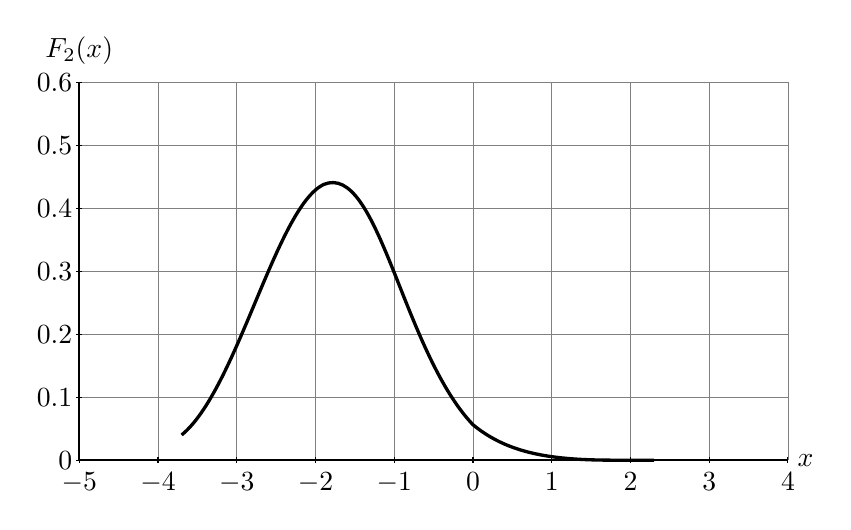
\begin{tikzpicture}
	%learn to try
	\draw[gray, very thin] (-5, 0) grid[xstep=1, ystep= 0.8] (4, 4.8);
	%axes
	\draw[thick] (-5, 0) -- (4, 0)
					(-5, 0) -- (-5, 4.8);
	\foreach \x in {-5, -4, -3 ,-2, -1, 0, 1, 2, 3, 4}
		\draw [xshift = \x cm] (0 pt, 1pt) -- (0 pt, -1pt) node[below] {$\x$};
	\foreach \y/\ytext in {0, 0.8/0.1, 1.6/0.2, 2.4/0.3, 3.2/0.4, 4.0/0.5, 4.8/0.6}
		\draw [xshift = -5 cm, yshift = \y cm] (-1pt, 0pt) -- (1pt, 0pt) node[left] {$\ytext$};
	\draw (4, 0) node[right] {$x$}
			(-5, 4.9) node[above] {$F_2(x)$};
	\draw[very thick] (-3.7, 0.32) .. controls (-3, 0.89) and (-2.5, 3.2) .. (-1.9, 3.5)
		   (-1.9, 3.5) .. controls (-1.2, 3.8) and (-0.9, 1.4) .. (0, 0.45)
		   (0, 0.45) .. controls (0.45, 0.08) and (1.0, 0) .. (1.8, 0)
		   (1.8, 0) -- (2.3, 0);
\end{tikzpicture}
\end{document}